\appendix
\clearpage % o \cleardoublepage
\addappheadtotoc
\appendixpage

\chapter{Manual de usuario}
\label{cap:manualUsuario}
Este apéndice es el manual de usuario del entorno interactivo.
Muestra la instalación de la aplicación y explica el funcionamiento de la misma.

\section{Instalación}
\label{sec:instalacion}
\par
El entorno interactivo no necesita de un proceso de instalación.
Se trata de un archivo \textit{JAR} (\textit{Java Archive}), lo que facilita la distribución de la aplicación.

\subsection{Requisitos mínimos}
\label{ssec:requisitos_minimos}
El requisito mínimo para la ejecución de la aplicación es:
\begin{itemize}
  \item Tener instalada la Máquina Virtual de Java (JVM) en su versión 1.6 o superior.\\
	Se puede obtener gratuitamente en: \texttt{http://www.java.com/es/download/index.jsp}
\end{itemize}

\section{Ejecución}
La aplicación se puede ejecutar simplemente haciendo doble clic sobre el fichero \textit{JAR}.
También es posible ejecutarlo desde un terminal de línea de comandos con la siguiente instrucción:
\texttt{java -jar <<aplicación.jar>>}

\section{Funcionamiento}
\label{sec:funcionamiento}
Tanto el aspecto de la aplicación como su funcionamiento son fáciles de entender. 
Todas la ventanas de la aplicación contienen en su parte inferior una zona dedicada a mostrar información de ayuda sobre el componente de la ventana en el que se sitúa el usuario con el puntero del ratón.

El programa dispone de una pantalla principal dividida en tres partes: los juegos, las estrategias y las funciones principales.
La figura~\ref{fig:ventana_principal} muestra la ventana principal.

\begin{figure}[!h]
	\centering
	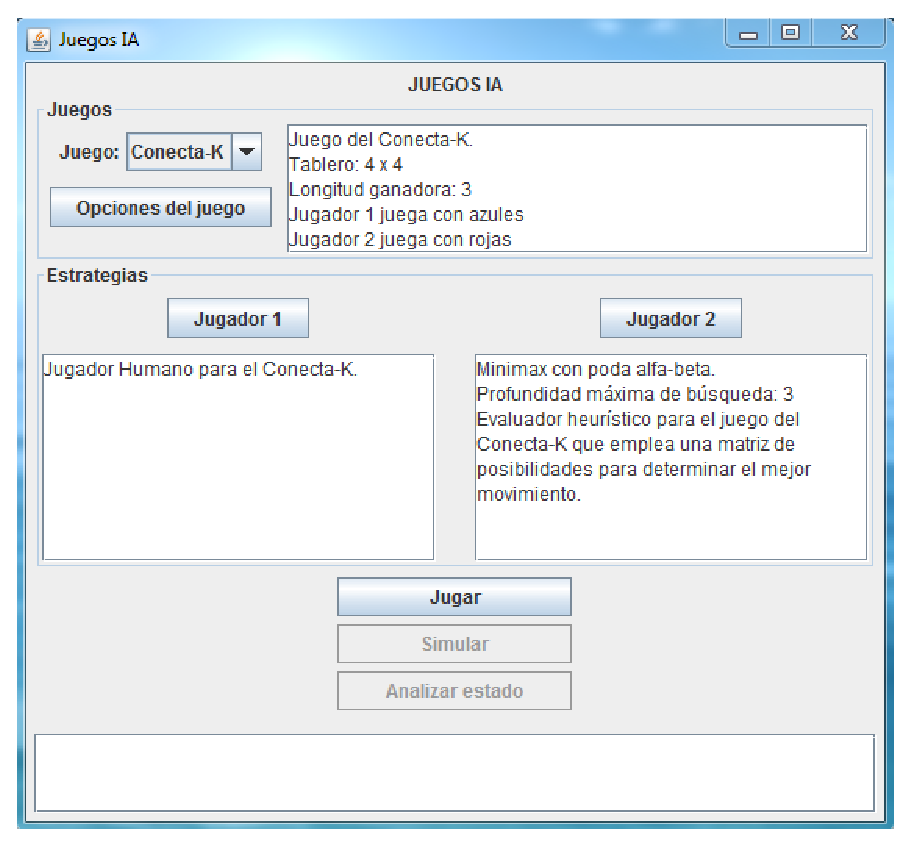
\includegraphics[scale=0.4]{contenido/apendiceA/imagenes/ventanaPrincipal.eps}
	\caption{Pantalla principal de la aplicación.}
	\label{fig:ventana_principal}
\end{figure}

La parte de los juegos nos permite seleccionar y configurar un juego; la parte de estrategias se encarga de seleccionar, configurar y entrenar si es necesario las estrategias de los dos jugadores y por último tenemos los tres modos de uso de la aplicación: jugar, simular y analizar estado.

Estas partes están organizadas de arriba a abajo, pues el orden de uso es importante: primero se debe elegir y configurar el juego, a continuación las estrategias de los dos jugadores y por último elegir la acción deseada.
Esto es así porque las estrategias pueden necesitar información del juego y este último debe estar configurado previamente.
Si seleccionamos un juego después de configurar las estrategias, las estrategias se restablecerán a sus valores por defecto.

\subsection{Selección y configuración del juego}
\label{ssec:funcionamiento_juegos}
Se puede seleccionar un juego directamente desde la pantalla principal de la aplicación; junto a él se muestra información del juego y su configuración por defecto.

Si se desea cambiar la configuración del juego debemos seleccionar la opción \texttt{``Opciones del juego''}.
Se accede a una nueva ventana con diferentes opciones de configuración que dependen del juego seleccionado.
Para obtener ayuda sobre estas opciones hay que situar el puntero del ratón sobre las mismas y se obtendrá información sobre ella en la parte inferior de la ventana.

\subsection{Selección y configuración de los jugadores}
\label{ssec:funcionamiento_jugadores}
La parte central de la ventana principal esta dividida a su vez en dos partes: una dedicada al primer jugador y otra al segundo jugador.
Cada una de ellas muestra información sobre la estrategia actual seleccionada para el jugador.
La estrategia por defecto es un jugador humano.
Pulsando los botones \texttt{``Jugador 1''} y \texttt{``Jugador 2''} podemos cambiar y configurar las estrategias para cada jugador.

La figura~\ref{fig:ventana_estrategia} muestra la ventana de configuración de las estrategias; esta ventana es idéntica para ambos jugadores.
Contiene una lista con las estrategias disponibles; al seleccionar una estrategia se muestra al lado información sobre la misma y la parte inferior de la ventana cambia para mostrar las opciones de configuración de esa estrategia.\footnote{No todas las estrategias son configurables.}

\begin{figure}[!h]
	\centering
	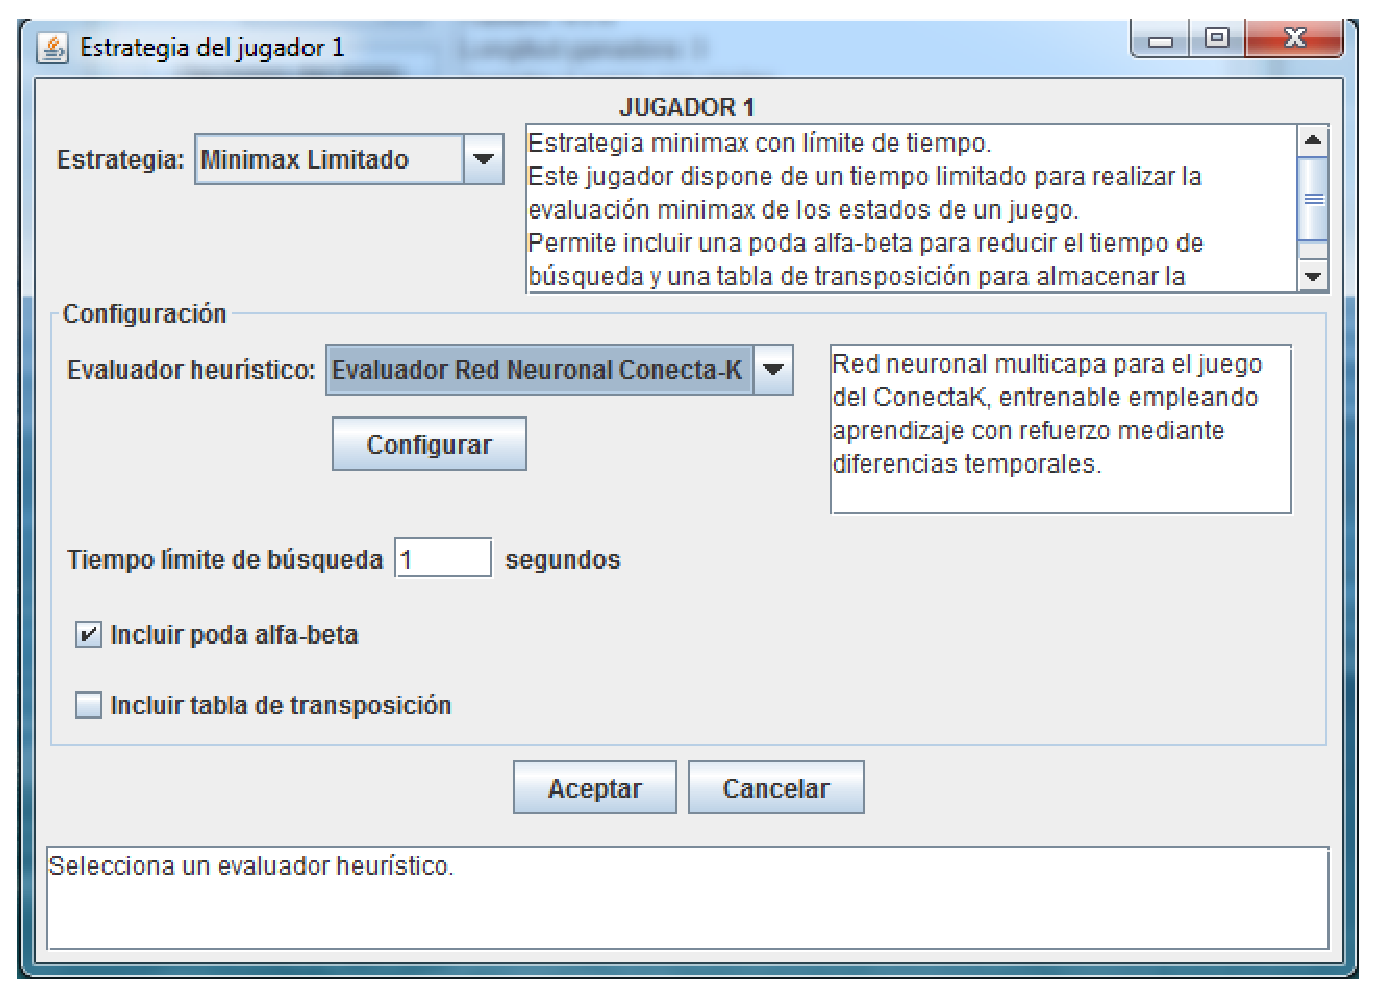
\includegraphics[scale=0.4]{contenido/apendiceA/imagenes/ventanaEstrategias.eps}
	\caption{Pantalla de selección y configuración de la estrategia.}
	\label{fig:ventana_estrategia}
\end{figure}

La opción más interesante es la selección y configuración de un evaluador heurístico para las estrategias.
Esta opción sólo estará disponible en las estrategias que necesiten de un heurístico para evaluar las posiciones de los juegos.
Por otro lado también hay heurísticos que no necesitan configurar sus parámetros.

En el caso de que el heurístico permita configurar sus parámetros se activa la opción \texttt{``Configurar''} debajo del heurístico seleccionado.
Esta opción da acceso a una nueva ventana como la que se muestra en la figura~\ref{fig:ventana_evaluador}.

\begin{figure}[!h]
	\centering
	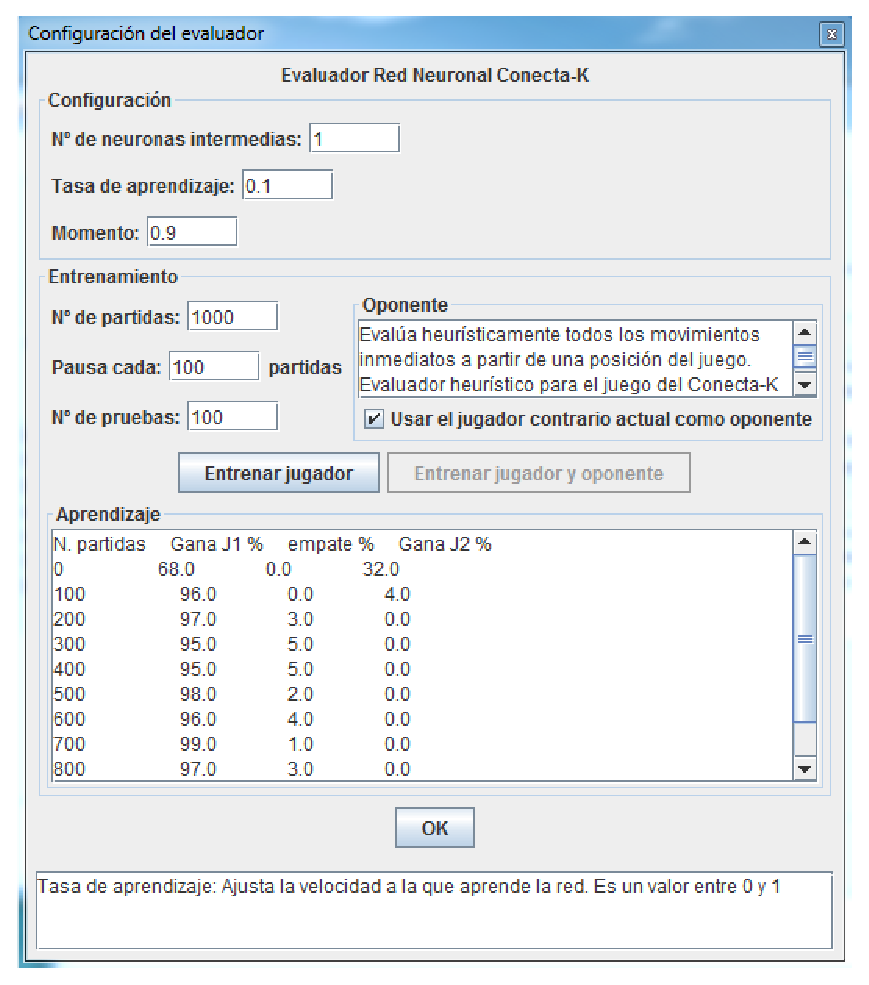
\includegraphics[scale=0.5]{contenido/apendiceA/imagenes/ventanaEvaluador.eps}
	\caption{Pantalla de configuración y entrenamiento de un evaluador heurístico.}
	\label{fig:ventana_evaluador}
\end{figure}

La parte superior muestra los parámetros de configuración del evaluador heurístico, mientras que la parte inferior permite entrenar el evaluador.
La parte de entrenamiento sólo se mostrará si el evaluador es entrenable; en caso contrario la ventana sólo mostrará los parámetros de configuración del evaluador.

\subsubsection{Entrenamiento del jugador}
\label{sssec:entrenamiento_jugador}
La ventana de configuración del evaluador permite entrenar al evaluador heurístico y por tanto al jugador usando aprendizaje por refuerzo.

La parte inferior de la ventana (figura~\ref{fig:ventana_evaluador}) muestra las opciones de entrenamiento.
Para entrenar al jugador se debe indicar el número de partidas de entrenamiento.
Los campos \texttt{``pausa cada \textit{n} partidas''} y \texttt{``número de pruebas''} permiten ver el desarrollo del aprendizaje.
Cada \textit{n} partidas de entrenamiento se realizará una pausa y se jugará el número de partidas de prueba indicado; el resultado de estas pruebas se irá mostrando en la parte inferior.

El entrenamiento se realiza por defecto frente a un oponente con estrategia aleatoria; pero también se puede entrenar frente al jugador contrario activando la opción \texttt{``Usar el jugador contrario actual como oponente''}.
Esta opción sólo se podrá activar si el jugador contrario es controlador por el ordenador, es decir, no es un jugador humano.

La misma ventana de entrenamiento también permite entrenar simultáneamente a los dos jugadores seleccionados.
Para ello el jugador contrario debe ser entrenable y debe activarse la opción \texttt{``Usar el jugador contrario actual como oponente''} comentada anteriormente.
Al activar esta opción aparece un nuevo botón \texttt{``Entrenar jugador y oponente''} que sólo estará activo si el jugador oponente también es entrenable.
Se entrenará simultáneamente a los dos jugadores, uno frente al otro, cada uno con su propia estrategia.

\subsection{Modos de uso de la aplicación}
\label{ssec:funcionalidad}
La aplicación tiene tres modos de uso básicos: jugar, simular y analizar estado.
A continuación se explica el funcionamiento de cada uno de estos modos.

\subsubsection{Jugar}
\label{sssec:jugar}
Esta opción nos permite jugar una partida al juego seleccionado.
Se puede jugar contra cualquier estrategia disponible o contra otro jugador humano.
En el caso de que ninguna de las estrategias sea un jugador humano, se mostrará el desarrollo de una partida entre los dos jugadores controlados por el ordenador.

La figura~\ref{fig:ventana_jugar} muestra el desarrollo de una partida de Go entre dos jugadores controlados por el ordenador.
La parte derecha muestra información sobre las estrategias y sobre el desarrollo de la partida (último movimiento, turno del jugador, puntuación,\ldots). La parte inferior muestra información sobre el movimiento actual, por ejemplo indicando si estamos sobre una posición sobre la que está prohibido mover.

\begin{figure}[!h]
	\centering
	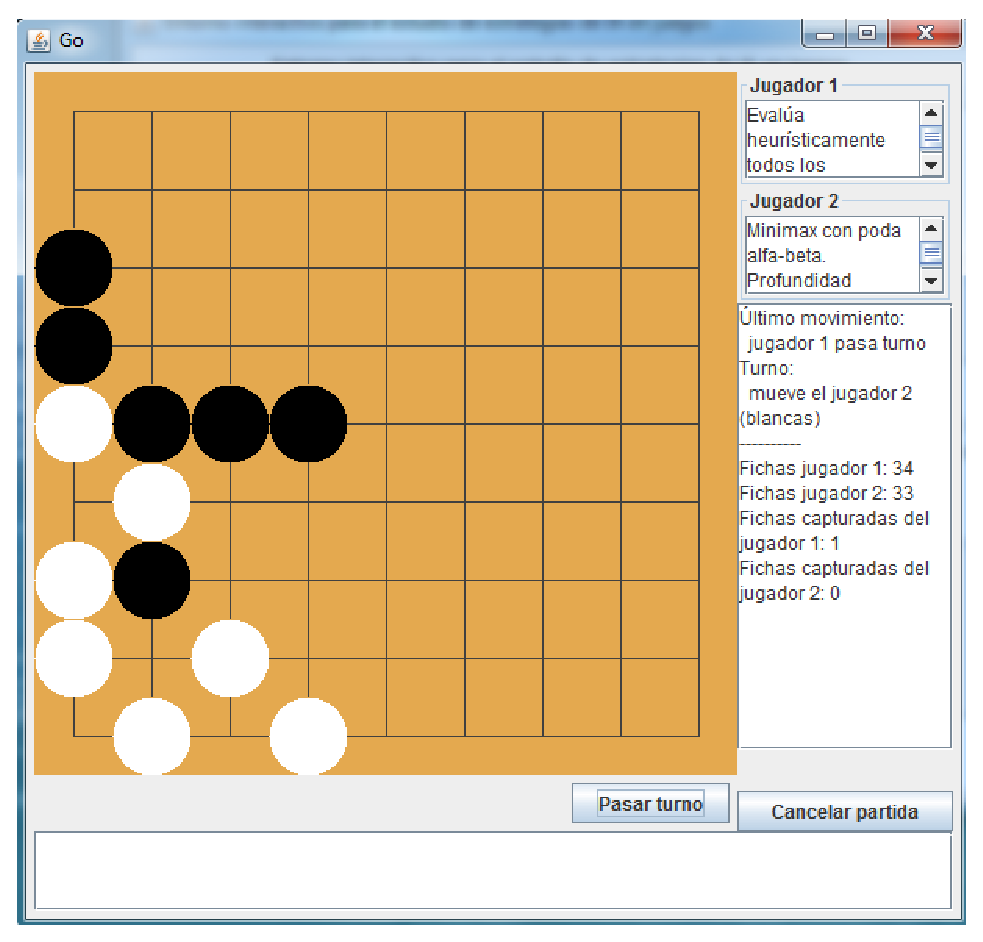
\includegraphics[scale=0.5]{contenido/apendiceA/imagenes/ventanaJuego.eps}
	\caption{Pantalla de juego.}
	\label{fig:ventana_jugar}
\end{figure}

Dependiendo de la estrategia usada, los movimientos de los jugadores pueden ser muy rápidos y el ojo humano no es capaz de seguir el desarrollo de la partida; para evitar esto se realiza una pequeña pausa de un segundo entre cada movimiento.
La partida puede cancelarse en cualquier momento, volviendo a la pantalla principal.

Cuando termina la partida se muestra la ventana de estadísticas con información acerca de la partida.

\subsubsection{Simular}
\label{sssec:simular}
La opción ``Simular'' consiste en realizar un número determinado de partidas entre dos jugadores controlados por el ordenador.
El desarrollo de estas partidas no es visible, pues el propósito de la simulación es comparar las estrategias con los resultados obtenidos a partir de todas las partidas jugadas.
La figura~\ref{fig:ventana_simulacion} muestra la ventana de simulación.

\begin{figure}[!h]
	\centering
	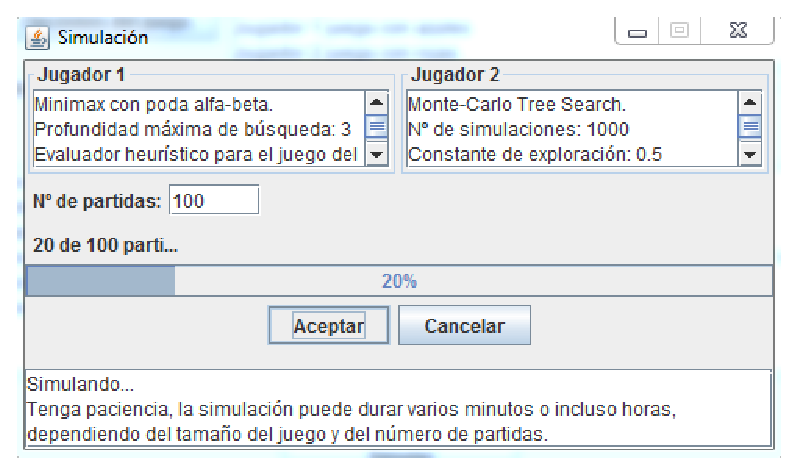
\includegraphics[scale=0.5]{contenido/apendiceA/imagenes/ventanaSimulacion.eps}
	\caption{Pantalla de simulación.}
	\label{fig:ventana_simulacion}
\end{figure}

Para realizar una simulación con éxito hay que tener en cuenta el tamaño del árbol de búsqueda del juego seleccionado y las estrategias elegidas porque una simulación puede durar desde segundos hasta horas, en función de estos factores y el número de partidas que se jueguen.
La simulación puede cancelarse en cualquier momento.
%En este caso no es posible detener la simulación una vez comenzada, pues se trata de un proceso intensivo en CPU y la interfaz queda deshabilitada.\footnote{Para cancelar una simulación se debe cerrar la aplicación desde un terminal de línea de comandos o mediante el administrador de tareas del sistema.}

Al finalizar la simulación se muestran las estadísticas de las partidas en una nueva ventana.

\subsubsection{Analizar estado}
\label{sssec:analizar_estado}
Esta opción permite al usuario construir un estado del juego seleccionado y a continuación estudiar el movimiento que realizaría cada uno de los jugadores en esa posición.

Para construir el estado el usuario debe realizar los movimientos oportunos de los dos jugadores, situando fichas en las posiciones deseadas pero siempre siguiendo las reglas del juego.
El usuario alternará los movimientos de ambos jugadores hasta conseguir el estado deseado.

La figura~\ref{fig:ventana_analisis} muestra la construcción de un estado para el juego del Conecta-4.
Una vez construido el estado deseado se debe pulsar la opción \texttt{``Analizar estado''} y los dos jugadores elegidos realizarán un movimiento; independientemente del turno del jugador, ambos jugadores realizan el mismo movimiento para comparar la decisión que toman las estrategias usadas por los jugadores.

\begin{figure}[!h]
	\centering
	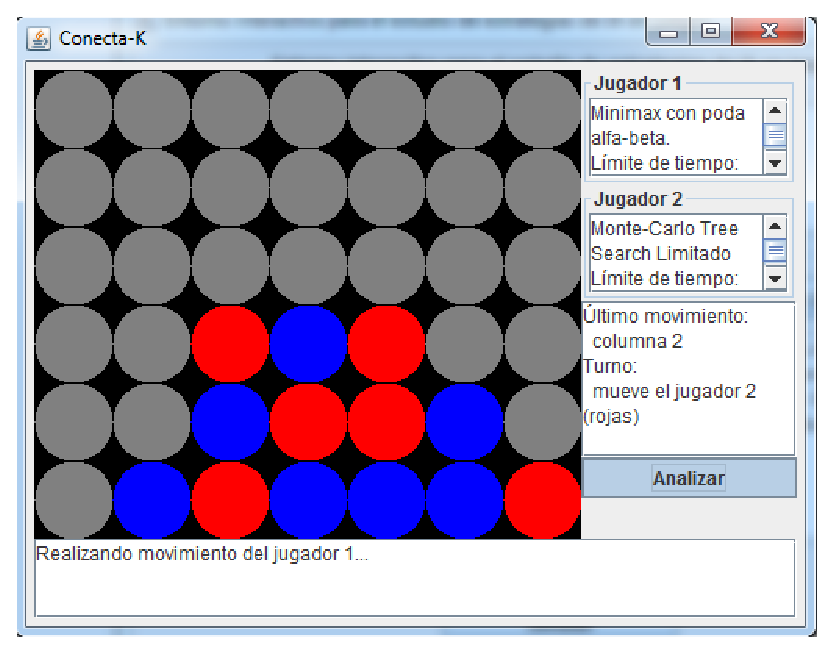
\includegraphics[scale=0.5]{contenido/apendiceA/imagenes/ventanaAnalisis.eps}
	\caption{Pantalla de análisis de estados.}
	\label{fig:ventana_analisis}
\end{figure}

Una vez finalizado el movimiento de los dos jugadores, se mostrará una nueva ventana con información de los movimientos realizados y estadísticas de las estrategias.

\subsection{Estadísticas}
\label{ssec:ventana_estadisticas}
Al finalizar cada uno de los modos de uso de la aplicación se mostrará una ventana con estadísticas.
La información mostrada en esta ventana depende del modo de uso elegido, aunque hay información común que es independiente del modo de uso y del jugador como el número de movimientos realizados o el tiempo medio de cada uno de los movimientos.

A continuación se describe brevemente la información mostrada para cada modo de uso de la aplicación:

\begin{description}
	\item[Jugar] (Figura~\ref{fig:subfig:ventana_estadisticas_jugar}) Al terminar de jugar una partida se muestra la situación del estado final, el último movimiento realizado, el resultado (el ganador), el tiempo de juego\footnote{El tiempo de juego incluye un segundo adicional por cada movimiento como se comentó en el apartado~\ref{sssec:jugar}.},\ldots
Los jugadores muestran estadísticas de sus estrategias para la partida completa.

	\item[Simular] (Figura~\ref{fig:subfig:ventana_estadisticas_simular}) En el caso de una simulación se muestra el porcentaje de partidas ganadas por cada jugador, el tiempo total de la simulación y el tiempo medio de cada partida.
Hay que prestar atención a la información mostrada por cada uno de los jugadores pues se trata de estadísticas acumuladas de todas las partidas.

	\item[Analizar estado] (Figura~\ref{fig:subfig:ventana_estadisticas_analizar}) Cuando termina el análisis se muestra el estado que ha sido analizado y los estados resultantes después de que los jugadores hayan movido.
	Cada estado puede mostrar información propia del mismo, aunque esta información depende del juego (último movimiento, puntuación actual de cada jugador,\ldots).
	Las estadísticas proporcionadas por los jugadores corresponden esta vez a un único movimiento.
	
\end{description}

\begin{figure}[h]
	\centering
	% Primera imagen
	\subfloat[]{
		\label{fig:subfig:ventana_estadisticas_jugar}
		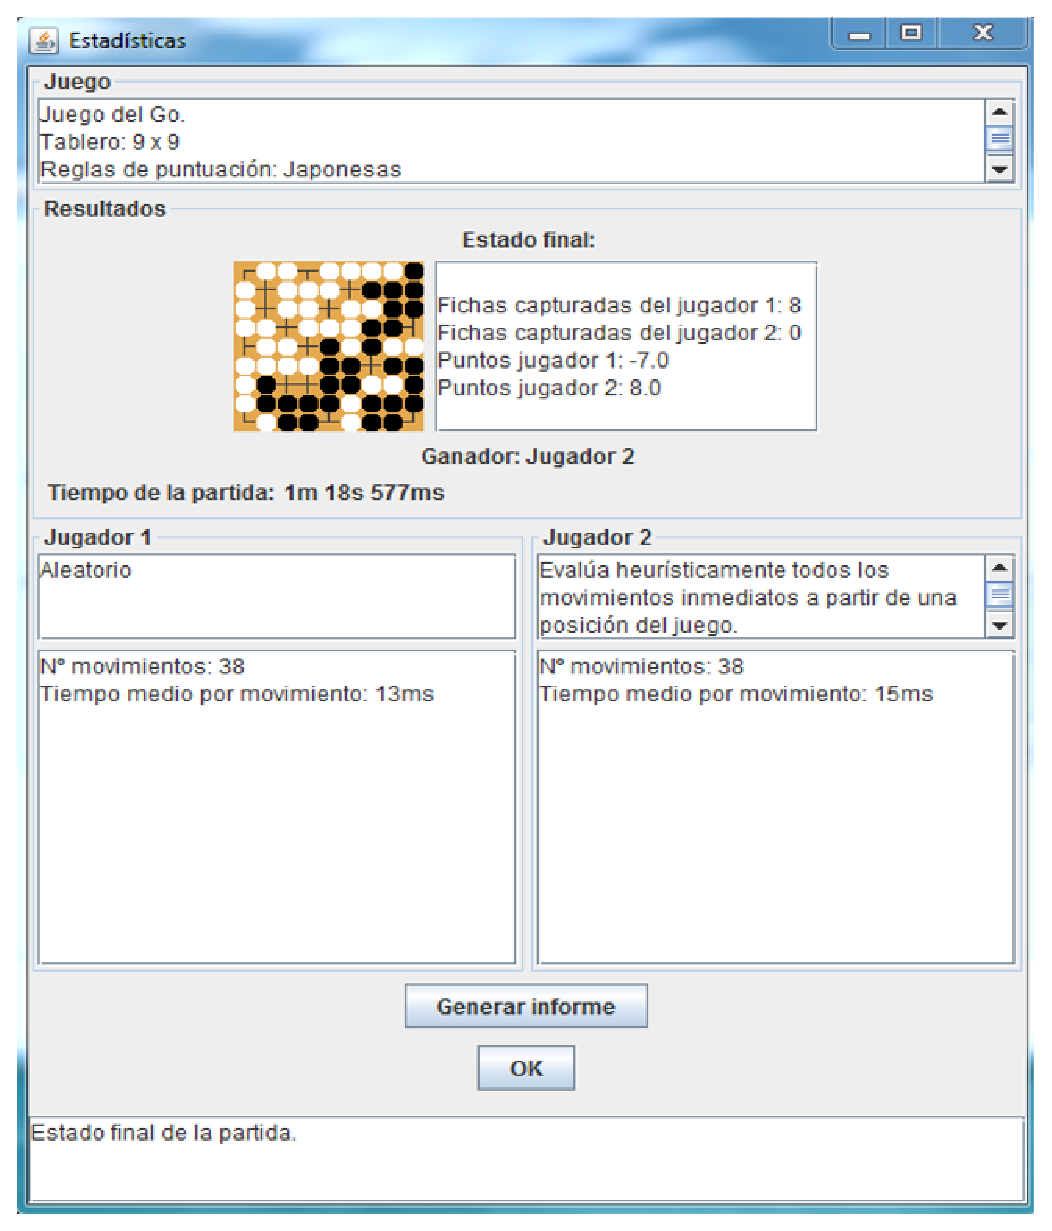
\includegraphics[scale=0.3]{contenido/apendiceA/imagenes/estadisticasJugar.eps}
	}
	\hspace{1cm}
	% Segunda imagen
	\subfloat[]{
		\label{fig:subfig:ventana_estadisticas_simular}
		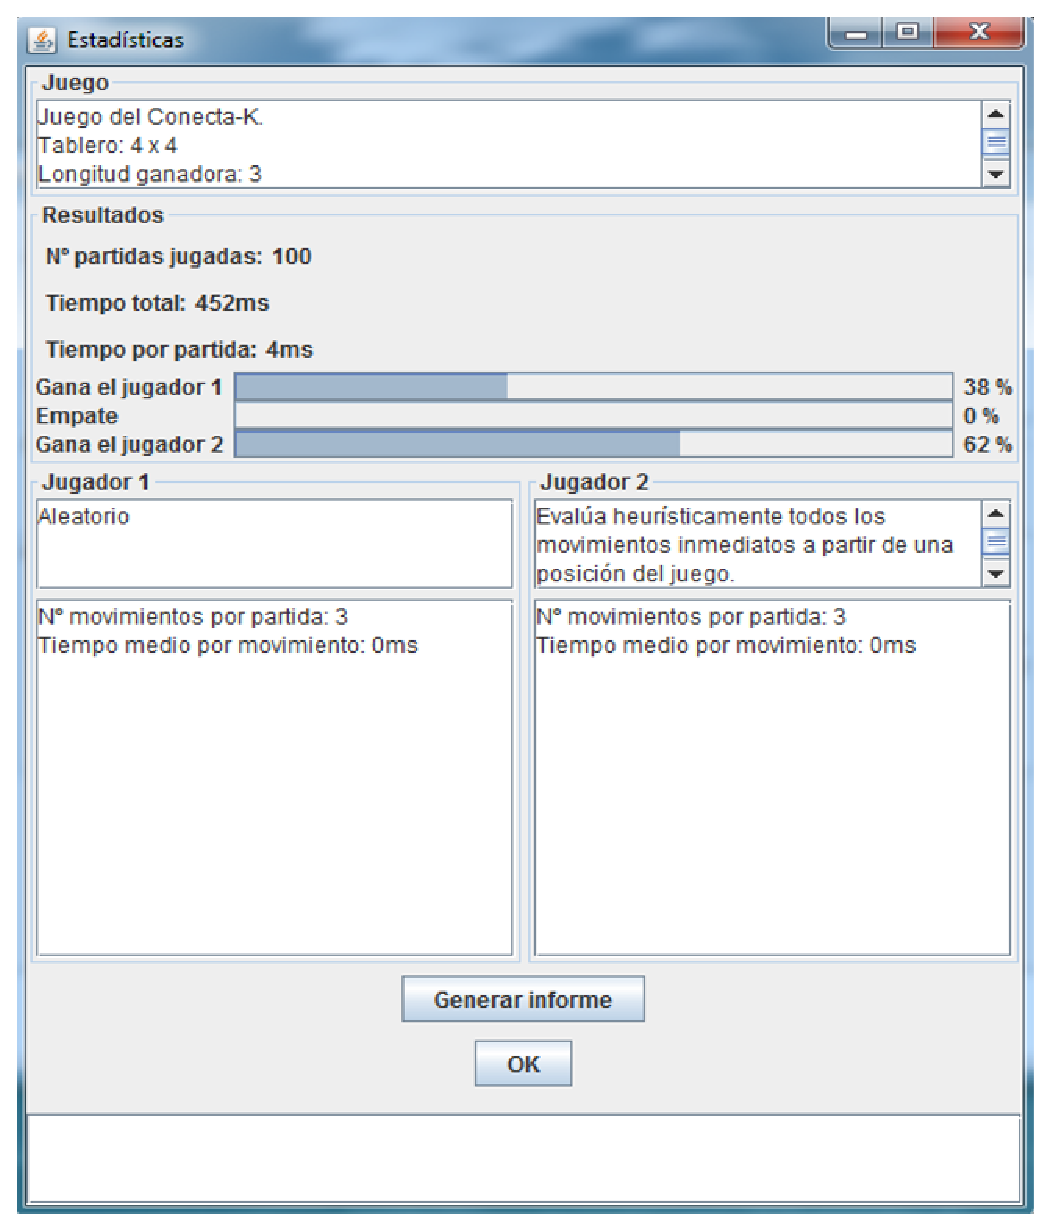
\includegraphics[scale=0.3]{contenido/apendiceA/imagenes/estadisticasSimulacion.eps}
	}
	\hspace{1cm}
	% Tercera imagen
	\subfloat[]{
		\label{fig:subfig:ventana_estadisticas_analizar}
		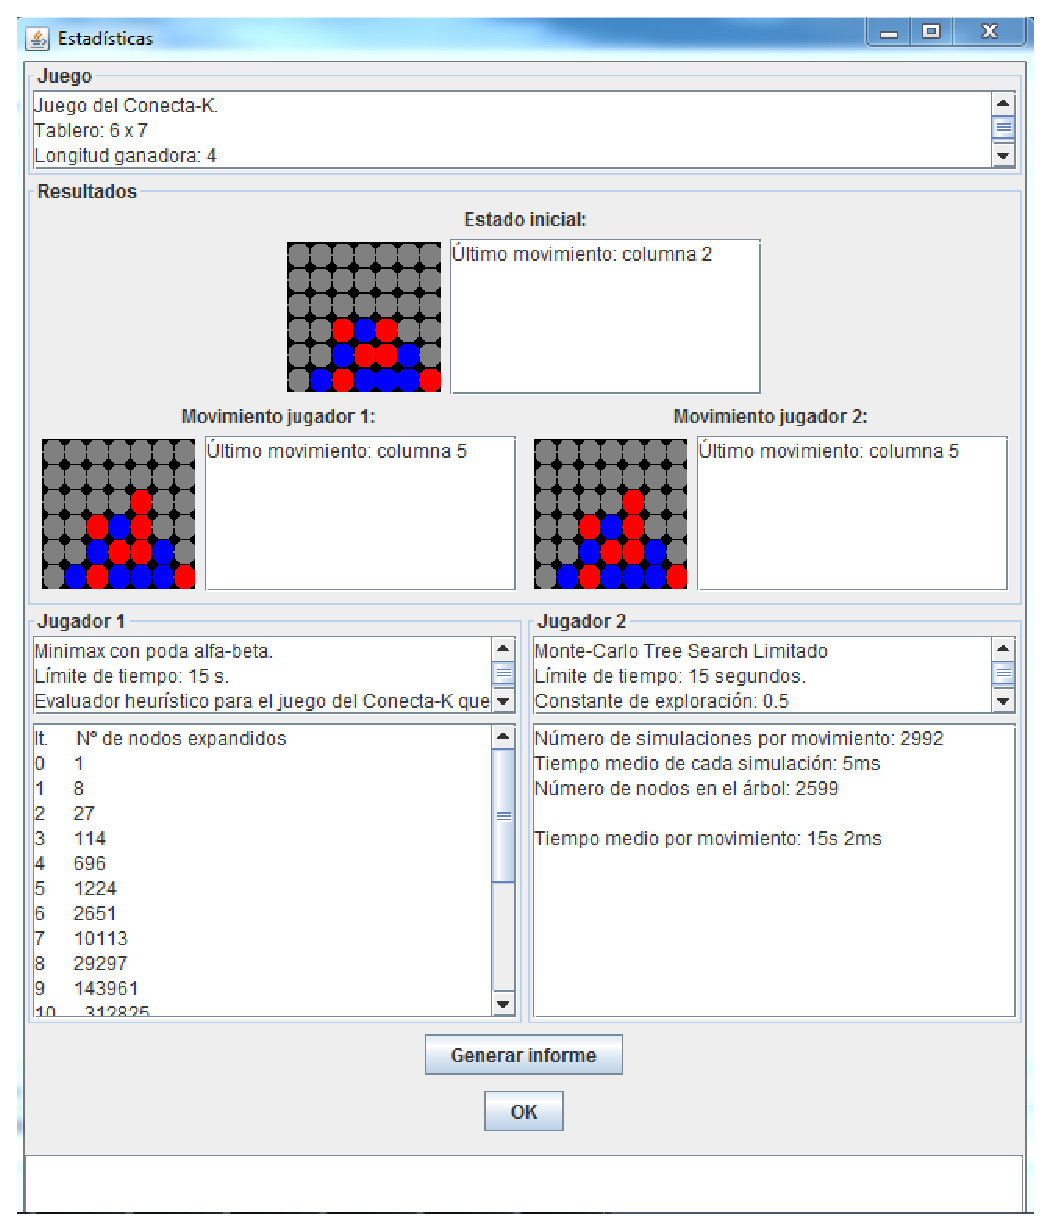
\includegraphics[scale=0.3]{contenido/apendiceA/imagenes/estadisticasAnalisis.eps}
	}
	\caption{Pantallas de resultados y estadísticas.}
	\label{fig:ventana_estadisticas}
\end{figure}

En todos los casos se puede generar un informe en formato texto plano con toda la información obtenida.
Para ello se debe seleccionar la opción \texttt{``Generar informe''}.









